\documentclass[compress]{beamer}

\usetheme{Berlin}

\usepackage{amsmath}
\usepackage{subcaption}
\usepackage{wrapfig}
\usepackage{multicol}
\usepackage[absolute,overlay]{textpos}
\usepackage{bibentry}
% \usepackage{pgfpages}
% \setbeamertemplate{note page}[plain]
% \setbeameroption{show notes on second screen=right}
% Required for including images
%\graphicspath{./media}

\usepackage{booktabs} % Top and bottom rules for tables

%\setbeamertemplate{footline}[frame number]

%\setbeamertemplate{headline}
%{%
%  \begin{beamercolorbox}[colsep=1.5pt]{upper separation line head}
%  \end{beamercolorbox}
%  \begin{beamercolorbox}{section in head/foot}
%    \vskip2pt\insertnavigation{\paperwidth}\vskip2pt
%  \end{beamercolorbox}%
%  \begin{beamercolorbox}[colsep=1.5pt]{lower separation line head}
%  \end{beamercolorbox}
%}

%\setbeamertemplate{section page}
%{
%    \begin{centering}
%    \begin{beamercolorbox}[sep=12pt,center]{part title}
%    \usebeamerfont{section title}\insertsection\par
%    \end{beamercolorbox}
%    \end{centering}
%}

\gdef\segmentName{}
\newcounter{Segment}
\setcounter{Segment}{0}
\newcommand{\finishSegment}{\label{endSegment\theSegment}}
\newcommand{\startSegment}[1]{
\label{beginSegment\theSegment}
\setcounter{framenumber}{1}
\stepcounter{Segment}
\gdef\segmentName{#1}
}

\setbeamertemplate{footline}
{
\hfill \segmentName\ \ %
\usebeamercolor[fg]{page number in head/foot}%
\usebeamerfont{page number in head/foot}%
\setbeamertemplate{page number in head/foot}{\insertframenumber\,/\,\inserttotalframenumber}
\setbeamertemplate{page number in head/foot}{\insertframenumber\,/\,\ref{endSegment\theSegment}}%
\usebeamertemplate*{page number in head/foot}\kern1em\vskip2pt%
}

\setbeamertemplate{section in toc}[default]
\setbeamertemplate{subsection in toc}[default]

\setbeamertemplate{bibliography item}{\insertbiblabel}

\title{Exploring the formation and robustness of partially relaxed MHD states}
\author{Matt Ketkaroonkul\inst{1}, Adelle Wright\inst{2}}
\institute{\raggedright
    \inst{1} University of Washington, Seattle\\
    \inst{2} Princeton Plasma Physics Laboratory\\
}
\date{Aug 16, 2022\\ PPPL SULI}
% \nobibliography*

\begin{document}

%\addtobeamertemplate{block end}{}{\vspace*{2ex}} % White space under blocks
%\addtobeamertemplate{block alerted end}{}{\vspace*{2ex}} % White space under highlighted (alert) blocks

%\setlength{\belowcaptionskip}{0ex} % White space under figures
%\setlength{\belowdisplayshortskip}{2ex} % White space under equations

\frame{\titlepage\thispagestyle{empty}}
\part{Introduction}
\frame{\startSegment{Introduction}\partpage}

\section{Introduction}
% To introduce my project, I would like to preface the issues that my project touches upon

\begin{frame}{Preface}
    \begin{itemize}
        \item Fusion plasmas are {\bf not ideal}
            \begin{itemize}
                \item Magnetic flux is not frozen-into the plasma
                \item Magnetic flux can form islands in non-ideal plasma
                \item and much more \ldots
            \end{itemize}

        \item Ideal MHD is thus not an accurate description of fusion plasma
    \end{itemize}
    \begin{figure}[htpb]
        \centering
        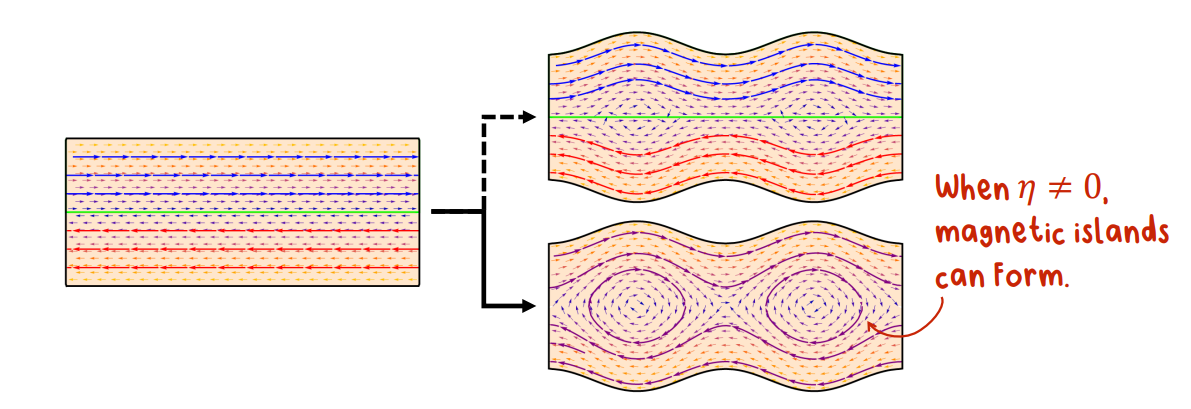
\includegraphics[scale=0.20]{media/magnetic-topology.png}
        \caption{Credit: "Introduction to MHD" SULI Intro Course 2021. \cite{introtomhd}}
    \end{figure}

\end{frame}

% add visual here or in above slide to demonstrate how flux changes topology depending on resistivity

\begin{frame}{Multiregion Relaxed MHD (MRxMHD)}
    \begin{itemize}
        \item A {\bf Multiregion Relaxed (MRx)} model is used instead
            \begin{itemize}
                \item Taylor relaxation occurs only within subregions of plasma \cite{dewar2017}
            \end{itemize}
        \item {\bf Taylor Relaxation}
            \begin{itemize}
                \item Process of plasma transitioning into lower energy state
            \end{itemize}
        \item {\bf Ideal Interfaces}
            \begin{itemize}
                \item Thin layers of ideal plasma
                \item Forms a current sheet structure
                \item In analysis, layers are assumed to have {\bf zero} thickness
            \end{itemize}
        \item {\bf Applications}
            \begin{itemize}
                \item Critical tool for optimizing stellarator design
                \item Model magnetic field perturbations in tokamaks
            \end{itemize}
    \end{itemize}

\end{frame}

\begin{frame}{Project Overview}
    Our project aims to test the {\bf robustness} of ideal interfaces in MRxMHD.
    % when we say robustness, we mean
    \begin{itemize}
        \item Testing the presence of interfaces in resistive plasma
        \item Typically expect current sheet structures to break down in resistive plasmas
    \end{itemize}
    
    This presentation will go over the following parts of the project:
    \begin{itemize}
        \item Mathematical Methods --- Boundary Layer Theory, Perturbation Methods % , Fourier Analysis
        \item Literature Analysis and Derivations
    \end{itemize}
    \finishSegment
\end{frame}

\part{Mathematical Methods}
\frame{\startSegment{Mathematical Methods}\partpage}

\section{Mathematical Methods}

\begin{frame}{Boundary Layer Theory \cite{benderorszag}}
    \begin{itemize}
        \item {\bf Boundary Layer} --- narrow region where DE solution ``changes rapidly''
            \begin{itemize}
                \item perturbing parameter $\varepsilon$ (generally small)
                \item characteristic size of narrow region $\delta$
            \end{itemize}
        \item {\bf Inner} and {\bf Outer} solutions \ldots
            \begin{itemize}
                \item approximate the actual solution
                \item {\bf inner} --- rapidly changing soln.
                \item {\bf outer} --- slowly changing soln.
                \item solutions may be ``stitched'' together with asymptotic matching
            \end{itemize}
        \item Motivation
            \begin{itemize}
                \item interest in MHD equilibrium at small resistivity $\eta$ (i.e. force balance in a plasma)
            \end{itemize}
    \end{itemize}
\end{frame}

\begin{frame}{Boundary Layer Theory --- Example \cite{benderorszag}}
    \begin{columns}
       \begin{column}{0.6\textwidth}
            Consider the following DE solution with $y(0)=0,\, y^\prime (1)=1$
            \begin{equation}
                \varepsilon y^{\prime\prime}+\left( 1+\varepsilon \right) y^\prime+y=0
            \end{equation} 
            \begin{equation}
                y(x)=\frac{e^{-x}-e^{-x / \varepsilon}}{e^{-1}-e^{-1 / \varepsilon}}
            \end{equation} 
            \begin{itemize}
                \item outer solution changes slowly at $1<\varepsilon$
                \item inner solution changes rapidly at  $0<\varepsilon<1$
            \end{itemize}
       \end{column} 
       \begin{column}{0.4\textwidth}
            \begin{figure}[htpb]
                \centering
                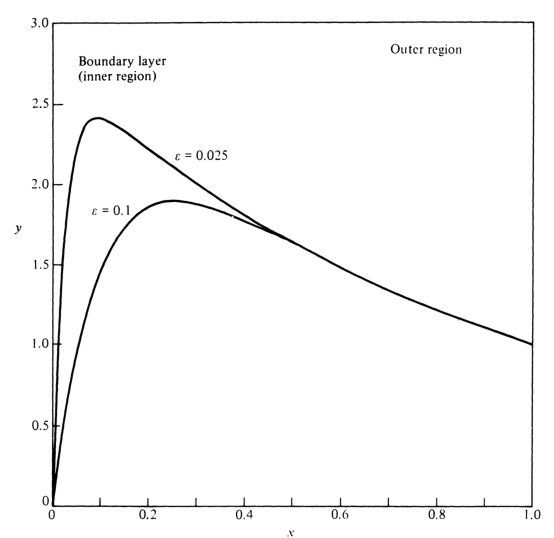
\includegraphics[scale=0.25]{media/inner-outer-solution.png}
            \end{figure}
       \end{column} 
    \end{columns}
\end{frame}

\begin{frame}{Perturbation Methods \cite{benderorszag}}
    Approximate a solution from an exact solution from a simpler problem
    \begin{itemize}
        \item Involved in linearizing PDEs
        % useful in finding solutions for notoriously non-linear MHD equations
        \item Express a solution in terms of a series expansion with small ``perturbing'' parameters
            \begin{equation}
                \psi=\sum_{n=0}^{\infty} \varepsilon^{n}\psi_n=\psi_0+\varepsilon\psi_1+\varepsilon^{2}\psi_2+\ldots
            \end{equation} 
        \item Can substitute variables within PDEs with series to get a system of equations, sorted by order of $\varepsilon$
        % an example of this will be shown in the literature review
        \item Assumptions made to eliminate certain terms
    \end{itemize}
    \finishSegment
\end{frame}

% Consider leaving some math methods slides out

\part{Literature Analysis and Derivations}
\frame{\startSegment{Literature Analysis and Derivations}\partpage}

\section{Literature Analysis and Derivations}

\begin{frame}{Dewar et al. (2017) \cite{dewar2017}}
    \begin{itemize}
        \item Description of magnetic flux under rippled boundary conditions
        \item ``HKT-Beltrami'' Slab Model
            \begin{itemize}
                \item Thin, annular section of a toroidal cross-section transformed into Cartesian coords.
                \item x-axis --- radial direction of toroidal cross-section
                \item y-axis --- poloidal direction. Periodic. $y \in [-\pi,\pi]$
            \end{itemize}
            % add visual here
        \item Slab boundaries are perturbed with ripples of amplitude $\alpha$

        \begin{figure}[htpb]
            \centering
            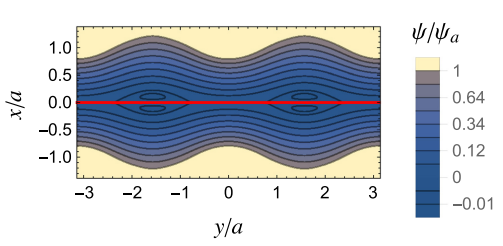
\includegraphics[scale=0.30]{media/dewar-boundary-ripples.png}
        \end{figure}
    \end{itemize}    
\end{frame}

\begin{frame}{Dewar et al. (2017) \cite{dewar2017}}
    The ansatz of the magnetic flux function is written as
    \begin{equation}
    \begin{split}
        \hat{\psi}_+ (x,y) & = c_0\cos{\mu x} + \sum_{l=1}^{\infty} c_{lm} \cos{\frac{lmy}{a}} \cosh{\kappa_{lm} x} \\
                           & + d_0 \sin{\mu x} + \sum_{l=1}^{\infty} d_{lm} \cos{\frac{lmy}{a}} \sinh{\kappa_{lm} x}
    \end{split} \end{equation} 
    The solution fits criterion such as:
    \begin{itemize}
        \item Helmholtz differential equation, $\left( \nabla^2 + \mu^2 \right) \hat{\psi}=0$
        \item Slab model geometry
    \end{itemize}
\end{frame}

\begin{frame}{Dewar et al. (2017) \cite{dewar2017}}
    There are two different boundary conditions we explored in the project
    \begin{enumerate}
        \item {\bf Bdy-1}
            \begin{equation}
                \label{eq:bdy1}
                \psi\left( \pm a, y \right) - \langle \psi\left( \pm a, y \right) \rangle = 2\alpha \psi_a \cos{k_y y}
            \end{equation} 
            \begin{itemize}
                \item boundary is described implicitly, generally easier to solve for
                \item accurate for small values of $\alpha$
            \end{itemize}
        \item {\bf Bdy-2}
            \begin{equation}
                \label{eq:bdy2}
                x_{\text{bdy}}\left( y \right) =a\left( 1-\alpha\cos{k_y y} \right) 
            \end{equation} 
            \begin{itemize}
                \item boundary is described explicitly as a function of position, difficult to solve for
                \item accurate for greater range of $\alpha$
            \end{itemize}

    \end{enumerate}
\end{frame}

\begin{frame}{Dewar et al. (2017) \cite{dewar2017}}
    \begin{itemize}
        \item {\bf Bdy-1}
        \[
            \psi\left( \pm a, y \right) - \langle \psi\left( \pm a, y \right) \rangle = 2\alpha \psi_a \cos{k_y y}
        \]
    \end{itemize}
    \vspace{-1.4em}
    \begin{columns}
        \begin{column}{0.5\textwidth}
            \begin{figure}[htpb]
                \centering
                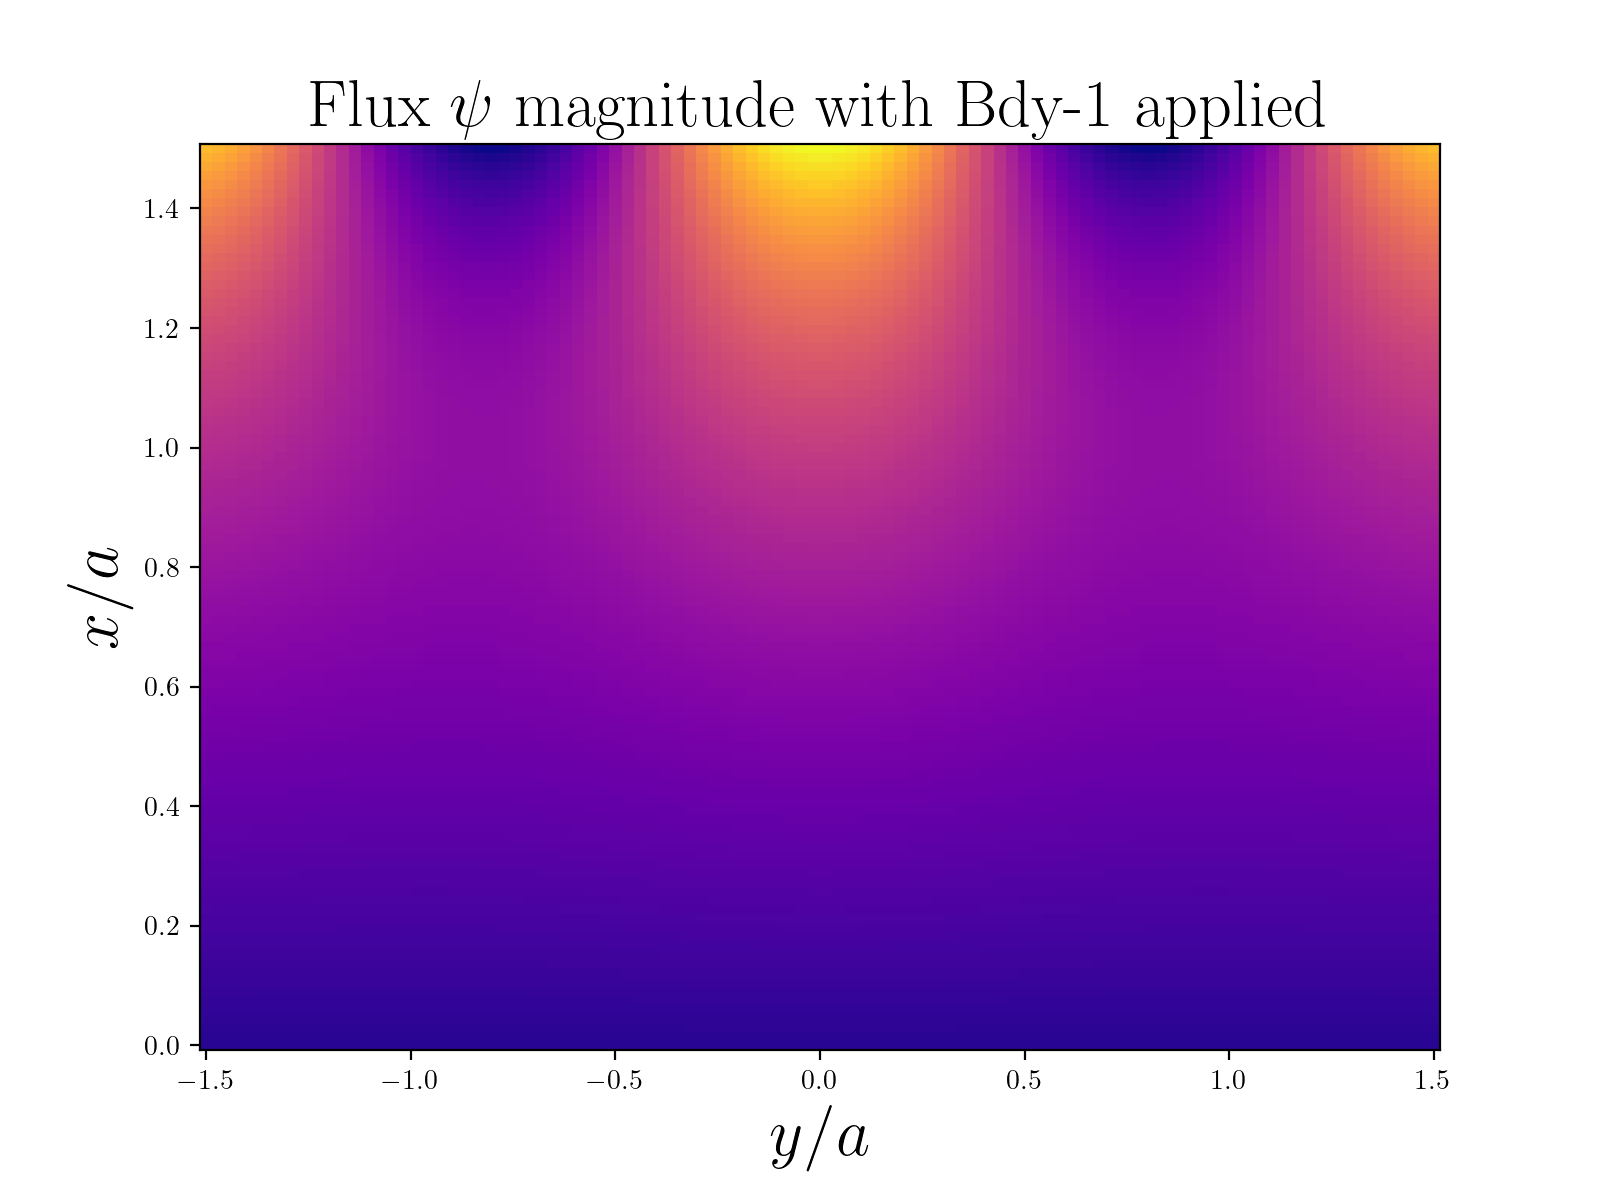
\includegraphics[scale=0.3]{media/bdy-1_general-solution.png}
                \caption{Plot of flux magnitude using Bdy-1}
            \end{figure}
       \end{column} 
       \begin{column}{0.5\textwidth}
            \begin{figure}[htpb]
                \centering
                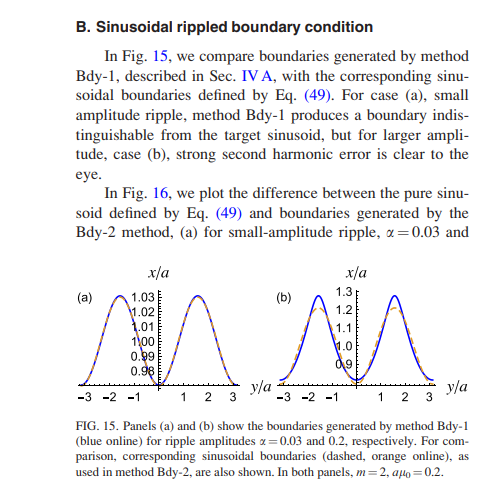
\includegraphics[scale=0.25]{media/dewar-bdy1-error.png}
                \caption{At larger values of $\alpha$ Bdy-1 ripples diverge from the actual.}
            \end{figure}
        \end{column}
    \end{columns}

\end{frame}

\begin{frame}{Dewar et al. (2017) \cite{dewar2017}}
    Applying equation (\ref{eq:bdy2}) for Bdy-2 involves substituting $x$ with
    \[
        x_{\text{bdy}}\left( y \right) =a\left( 1-\alpha\cos{k_y y} \right) 
    \]
    \begin{itemize}
        \item The solution involves compositions of sinusoidal functions, ex. $\cos(\mu a(1-\alpha\cos{k_y y}))$
        \item Two approaches:
            \begin{itemize}
                \item Expansion of the nested sinusoidals into a series of Bessel functions % in progress
                \item Taylor Expansion with respect to $\alpha$, truncating terms $\sim O(\alpha^2)$ and higher
            \end{itemize}
    \end{itemize}
\end{frame}


\begin{frame}{Wang, Bhattacharjee (1992) \cite{wangbhattacherjee}}
   \begin{itemize}
       \item Provides insight on timescales
           \begin{itemize}
               \item Phases A-D describe temporal evolution of a boundary-deformed magnetic field
               \item Exponential weighting of Alfven $\tau_A$ and Resistive $\tau_R$ timescales (generally $\tau_A < \tau_R$)
           \end{itemize}
        \item {\bf Insight} --- resistive effects and timescales become more significant with time
   \end{itemize} 
   \vspace{1em}
   \begin{columns}
       \begin{column}{0.6\textwidth}
           \begin{tabular}{|l|l|l|}
                \hline
                    & $\tau_A$ (ideal) & $\tau_R$ (non-ideal) \\
                \hline
                    Phase A & 2/3 & 1/3 \\
                \hline
                    Phase B & 2/5 & 3/5 \\
                \hline
                    Phase C & 1/2 & 1/2 \\
                \hline
                    Phase D & 1/4 & 3/4 \\
                \hline
            \end{tabular}
       \end{column}

       \begin{column}{0.4\textwidth}
           \begin{equation}
                \tau=\tau_A^{(1-s)}\tau_R^s
           \end{equation} 
       \end{column}
   \end{columns}
\end{frame}

\begin{frame}{Hahm, Kulsrud (1985) \cite{hahmkulsrud}}
    The following equation is a combination of the induction (with resistivity) and the fluid momentum conservation equations:
    \begin{equation}
        \label{eq:hk15}
        \frac{\partial \psi}{\partial t} + \vec{V}\cdot \vec{\nabla}\psi=\frac{\eta}{4\pi}\nabla^2 \psi
    \end{equation} 
    where
    \begin{itemize}
        \item $\vec{V}=\hat{z}\times \vec{\nabla}\phi$
        \item $\psi$ --- magnetic flux where $\vec{B}=B_T \hat{z}+\hat{z}\times \nabla \psi$ ($B_T$ is the toroidal magnetic field)
    \end{itemize}
\end{frame}

\begin{frame}{Hahm, Kulsrud (1985) \cite{hahmkulsrud}}

    Expanding (\ref{eq:hk15}) with a perturbation series and sorting terms by order of $\varepsilon$,
    \begin{equation}
        \label{eq:hkorder0}
        \varepsilon^0: \frac{\partial \psi_0}{\partial t} +\vec{V_0}\cdot \vec{\nabla}\psi_0=\frac{\eta}{4\pi}\nabla^2 \psi_0
    \end{equation} 
    \begin{equation}
        \label{eq:hkorder1}
        \varepsilon^1: \frac{\partial \psi_1}{\partial t} +\vec{V_0}\cdot \vec{\nabla}\psi_1+\vec{V_1}\cdot \vec{\nabla}\psi_0=\frac{\eta}{4\pi}\nabla^2 \psi_1
    \end{equation} 
    \begin{equation}
        \label{eq:hkorder2}
        \varepsilon^2: \frac{\partial \psi_2}{\partial t} +\vec{V_0}\cdot \vec{\nabla}\psi_2+\vec{V_1}\cdot \vec{\nabla}\psi_1+\vec{V_2}\cdot \vec{\nabla}\psi_0=\frac{\eta}{4\pi}\nabla^2 \psi_2
    \end{equation} 
\end{frame}

\begin{frame}{Hahm, Kulsrud (1985) \cite{hahmkulsrud}}
   Assumptions made with the equations:
   \begin{itemize}
       \item Let $\vec{V_0}=0$, making $\phi_0$ an arbitrary constant
       \item $\eta / 4\pi \sim O\left( \varepsilon^2 \right)$. This allows equations (\ref{eq:hkorder0}) and (\ref{eq:hkorder1}) to be equal to 0
   \end{itemize} 
   Which results in this equation,
   \begin{equation}
       \frac{\partial \psi_1}{\partial t} -kB_0 \frac{x}{a}\phi_1(x)=0
   \end{equation} 
   \begin{itemize}
       \item $k$ --- wave number
       \item $B_0$ --- the maximum magnetic field along the y-component
       \item $a$ --- characteristic spatial size of the system
       \item The partial derivative of phi is evaluated near $x=0$
   \end{itemize}
   \finishSegment
\end{frame}


\part{Summary and Goals}
\frame{\startSegment{Summary and Goals}\partpage} \section{Summary and Goals}
\begin{frame}{Summary of Findings}
    \begin{itemize}
        \item In the Dewar et al. paper; the solution found in this project for Bdy-2 via Taylor series approximation has modes $l=1,2$, as opposed to just $l=1$ as stated in the paper
        \item In the Wang, Bhattacharjee paper; resistive timescales become more dominant in determining the overall char. timescale as the plasma evolves over time
    \end{itemize} 
\end{frame}

\begin{frame}{Future Work}
   \begin{itemize}
       \item Continue work on solutions in the Dewar et al. paper under Bdy-2
           \begin{itemize}
               \item also comparing results between Bdy-1 and Bdy-2 under more scrutiny
           \end{itemize}
        \item Test flux functions on the linearized PDEs presented in Hahm, Kulsrud paper
       \item Begin work on nondimensionalization of DEs, giving more insight on when resistive timescale is non-negligible
   \end{itemize} 
    \finishSegment
\end{frame}

\part{References}
\frame{\startSegment{References}\partpage}

\section{References}

\begin{frame}{References}
    \begin{textblock*}{0.96\paperwidth}(0.02\paperwidth,0.1\paperwidth)
    \begin{multicols}{3}
    \fontsize{5}{6}
    \bibliographystyle{abbrv}
    \bibliography{bibliography.bib}
    \end{multicols}
    \end{textblock*}
    \finishSegment
\end{frame}

\part{Supplements}
\frame{\startSegment{Supplements}\partpage}

\section{Supplements}

\begin{frame}{Fourier Analysis \cite{benderorszag}}
Magnetic flux solutions can have the form similar to
\begin{equation}
    \sum_{n=1}^{\infty} C_n \sin\left( n\pi y / a \right) = V_0(y)
\end{equation} 
To determine coefficient $C_n$, multiply equation by $\sin\left( n^\prime \pi y / a \right)$ and integrate from $0$ to $a$ \cite{griffiths},
\begin{equation}
    \sum_{n=1}^{\infty} C_n \int_0^a \sin\left( n\pi y / a \right) \sin\left(   n^\prime \pi y / a \right)\, dy = \int_{0}^{a} V_0(y) \sin\left(   n^\prime \pi y / a \right)\, dy
\end{equation} 
\end{frame}

\begin{frame}{Fourier Analysis}
    The LH integral contains mutually orthogonal functions, which evalutates to
    \begin{equation}
        \int_0^a \sin\left( n\pi y / a \right) \sin\left(   n^\prime \pi y / a \right)\, dy = \frac{a}{2}\delta_{nn^\prime}
    \end{equation} 
    The coefficient is thus
    \begin{equation}
        C_n=\frac{2}{a}\int_{0}^{a} V_0(y)\sin\left( n \pi y / a \right)\, dy 
    \end{equation} 
\end{frame}

\begin{frame}{Dewar et al. Solutions}
Bdy-1 applied:
\begin{equation}
\begin{split}
    \hat{\psi}_+ (x,y) & = -\overline{\psi}\cos{\mu x} \\
                       & + \frac{2\alpha \psi_a}{\sinh{\kappa_m a}} \sinh{\kappa_m x} \cos\left( \frac{my}{a} \right) \\
                       & + \frac{2\alpha \psi_a \gamma_s \kappa_m}{\mu \sinh\left( \kappa_m a \right) } \sin\left( \mu x \right) 
\end{split}
\end{equation}
\end{frame}

\begin{frame}{Dewar et al. Solutions}
Bdy-2 applied:
\begin{equation}
    \begin{split}
        \hat{\psi}_+ (x,y) & = -\overline{\psi}\cos{\mu x} \\
                           & + \frac{\sin{\mu x}}{\sin{\mu a}} \left[\psi_a - \overline{\psi} - \frac{\overline{F}}{\mu}\left( 1+\cos{\mu a} \right) + \overline{\psi}\cos{\mu a} \right] \\
                           & + \overline{F}\alpha a \sin{\mu a} \sum_{l=1}^{2} \cos\left( \frac{lmy}{a} \right) \frac{\sinh{\kappa_{lm} x}}{\sinh{\kappa_{lm} a}}
    \end{split}
\end{equation} 
\end{frame}

\begin{frame}{Hahm, Kulsrud (1985) \cite{hahmkulsrud}}
    \begin{itemize}
        \item Description of inner and outer magnetic flux solution
        \item Outer Solution
        \begin{equation}
            \psi_1(x) = B_0\delta\left( \frac{\sinh{kx}}{\sinh{ka}} \right) 
        \end{equation} 
        \item Inner Solution
            \begin{equation}
                \xi=\frac{2}{\pi}\frac{B_0 k\delta}{\sinh{ka}}\int_{0}^{kxt / \tau_A}\frac{\sin{u}}{u}\, du  
            \end{equation} 
        where $\xi=\frac{\psi_1}{x}$
    \end{itemize}
    \finishSegment
\end{frame}

\end{document}
